\documentclass[final,t]{beamer}
\mode<presentation>
{
%  \usetheme{Warsaw}
%  \usetheme{Aachen}
%  \usetheme{Oldi6}
%  \usetheme{I6td}
  \usetheme{I6dv}
%  \usetheme{I6pd}
%  \usetheme{I6pd2}
}
% additional settings
\setbeamerfont{itemize}{size=\normalsize}
\setbeamerfont{itemize/enumerate body}{size=\normalsize}
\setbeamerfont{itemize/enumerate subbody}{size=\normalsize}

% additional packages
\usepackage{times}
\usepackage{amsmath,amsthm, amssymb, latexsym}
\usepackage{exscale}
%\boldmath
\usepackage{booktabs, array}
%\usepackage{rotating} %sideways environment
\usepackage[english]{babel}
\usepackage[latin1]{inputenc}
\usepackage[orientation=landscape,size=custom,width=200,height=120,scale=1.9]{beamerposter}
\listfiles
\graphicspath{{../graphics/}}
% Display a grid to help align images
%\beamertemplategridbackground[1cm]
 
\title{\huge Verification of the Neutron Mirror Capabilities in MCNPX via Gold Foil Measurements at the EIGER Instrument Beamline at the Swiss Spallation Neutron Source (SINQ) } %\thanks{Supported by Swiss National Science Foundation grant 200021\_150048/1}
\author{R.M. Bergmann, U. Filges, S. Forss, D. Reggiani, E. Rantsiou, T. Reiss, U. Stuhr, V. Talanov, M. Wohlmuther} %\thanks{ryan.bergmann@psi.ch}
\institute[PSI]{Paul Scherrer Institut, Villigen, Switzerland}
\date[May 7th, 2015]{May 7th, 2015}

% abbreviations
\usepackage{xspace}
\makeatletter
\DeclareRobustCommand\onedot{\futurelet\@let@token\@onedot}
\def\@onedot{\ifx\@let@token.\else.\null\fi\xspace}
\def\eg{{e.g}\onedot} \def\Eg{{E.g}\onedot}
\def\ie{{i.e}\onedot} \def\Ie{{I.e}\onedot}
\def\cf{{c.f}\onedot} \def\Cf{{C.f}\onedot}
\def\etc{{etc}\onedot}
\def\vs{{vs}\onedot}
\def\wrt{w.r.t\onedot}
\def\dof{d.o.f\onedot}
\def\etal{{et al}\onedot}
\makeatother




%%%%%%%%%%%%%%%%%%%%%%%%%%%%%%%%%%%%%%%%%%%%%%%%%%%%%%%%%%%%%%%%%%%%%%%%%%%%%%%%%%%%%%%%%%%%%%%%%%%%%%%%%%%%
%%%%%%%%%%%%%%%%%%%%%%%%%%%%%%%%%%%%%%%%%%%%%%%%%%%%%%%%%%%%%%%%%%%%%%%%%%%%%%%%%%%%%%%%%%%%%%%%%%%%%%%%%%%%
\begin{document}
\begin{frame}{} 
  \begin{columns}[t]
    \begin{column}{.3\linewidth}

      %%%%%%%%%%%%%%%%%%%%%%%%%%%%%%%%%%%%%%%%%%%%%%%%%%%%%%%%%%%%%%%%%%%%%%%%%%%%%%%%%%%%%%%%%%%%%%%%%%%%%%%%%%%%

      \begin{block}{Introduction}
        \begin{itemize}
        \item automatic sign language recognition system                                    %what
        \item \alert{necessary for communication} between deaf and
          hearing people
        \item \alert{continuous} sign language recognition,
          \alert{several} speakers, \alert{vision-based} approach, \alert{no
            special hardware}
        \item large vocabulary speech recognition (LVSR) system to
          obtain a textual representation of the signed
          sentences 
        \item evaluation of speech recognition techniques on \alert{publicly
          available sign language
          corpus}
        \end{itemize}

        \begin{equation}\label{eq:ref}
            R(Q) = 
            \begin{cases}
                Q > Q_c;  \qquad \frac{R_0}{2}\left\{  1 - \tanh\left(  \frac{Q - m Q_c}{W}\right) \right\}\{1-\alpha(Q-Q_c)\} \\
                Q \leq Q_c; \qquad R_0 \\
            \end{cases}
        \end{equation}

        pic of reflectivity curve?

      \end{block}

      %%%%%%%%%%%%%%%%%%%%%%%%%%%%%%%%%%%%%%%%%%%%%%%%%%%%%%%%%%%%%%%%%%%%%%%%%%%%%%%%%%%%%%%%%%%%%%%%%%%%%%%%%%%%
      
      \begin{block}{Gold Foil Measurement}
        \begin{columns}[T]
          \begin{column}{.75\linewidth}
            The vertical array of six gold foils shown in Figure \ref{foils} were exposed to the EIGER beam in December, 2013.   The foils were placed near the monochromator position at EIGER.  The foils are 25 mm in diameter and 30 mm center-to-center.  The blue marker lines in the figure show the approximate extent of the neutron guide.  The average current on the SINQ target during the irradiation was $200 \mu A$, and the foils were exposed for 5 minutes.  After irradiation, activation analysis was performed using a gamma spectrometer.
          \end{column}
          \begin{column}{.25\linewidth}
            \includegraphics*[width=\linewidth]{foils.eps}
          \end{column}
        \end{columns}
      \end{block}

      %%%%%%%%%%%%%%%%%%%%%%%%%%%%%%%%%%%%%%%%%%%%%%%%%%%%%%%%%%%%%%%%%%%%%%%%%%%%%%%%%%%%%%%%%%%%%%%%%%%%%%%%%%%%
      \begin{block}{MCNPX Geometry}
        \begin{columns}[t]
          \begin{column}{.75\linewidth}
            \noindent{\hskip1cm\textbf{Database}}
            \begin{itemize}
            \item system evaluation on the RWTH-BOSTON-104 database
              \begin{itemize}
              \item \alert{201 sentences} (161 training and 40 test sequences)
              \end{itemize}
            \end{itemize}

            \vskip1ex            
            \noindent{\hskip1cm\textbf{Problems}}
            \begin{itemize}
            \item 26\% of the training data are \alert{singletons}
            \end{itemize}

            \vskip1ex            
            \noindent{\hskip1cm\textbf{Differences in Comparison to ASR}}
            \begin{itemize}
            \item simultaneousness                       % multi-channel ... but unclear if necessary
            \end{itemize}
          \end{column}

          \begin{column}{.25\linewidth}
                 
          \end{column}
        \end{columns}

      \end{block}


      \end{column}

      %%%%%%%%%%%%%%%%%%%%%%%%%%%%%%%%%%%%%%%%%%%%%%%%%%%%%%%%%%%%%%%%%%%%%%%%%%%%%%%%%%%%%%%%%%%%%%%%%%%%%%%%%%%%


    \begin{column}{.3\linewidth}
      \begin{block}{Variance Reduction}
       

      \end{block}

    \end{column}

    %%%%%%%%%%%%%%%%%%%%%%%%%%%%%%%
    
    \begin{column}{.3\linewidth}

      \begin{block}{Experimental \vs Calculated Results}
        %%%%%%%%%%%%%%%%%%%%%%%%%%%%%%%%%%%%%%%%%%%%%%%%%%%%%%%
        \centering
        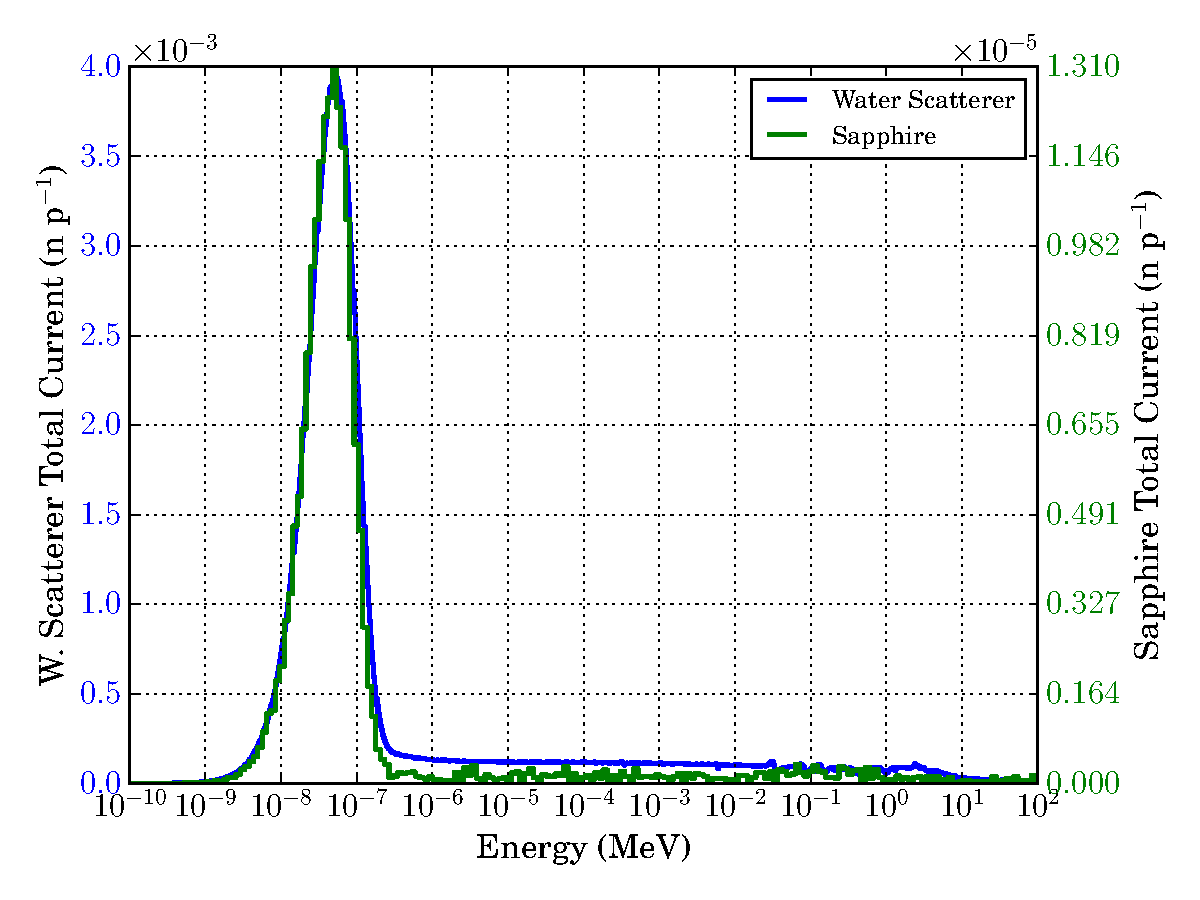
\includegraphics[width=0.33\linewidth]{specs.pdf}%
        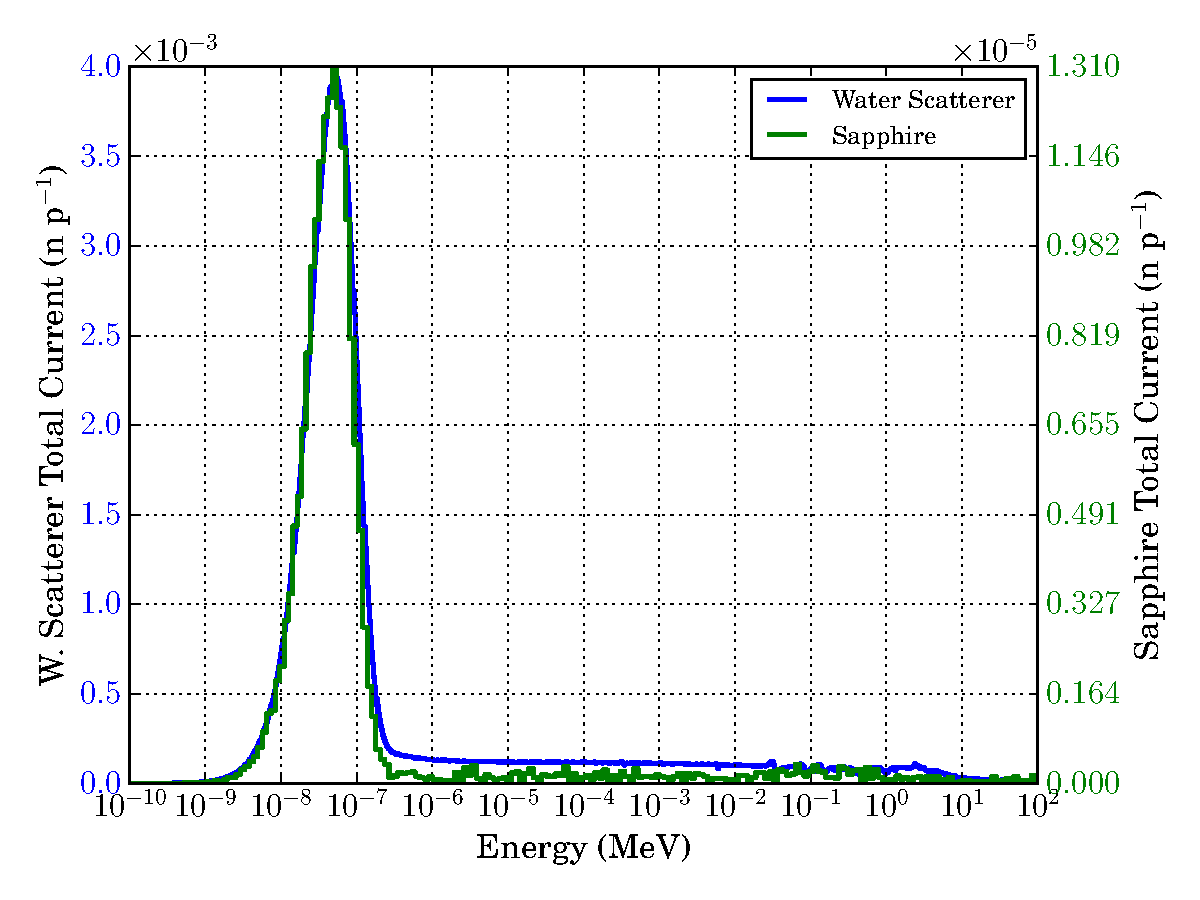
\includegraphics[width=0.33\linewidth]{specs.pdf}%
        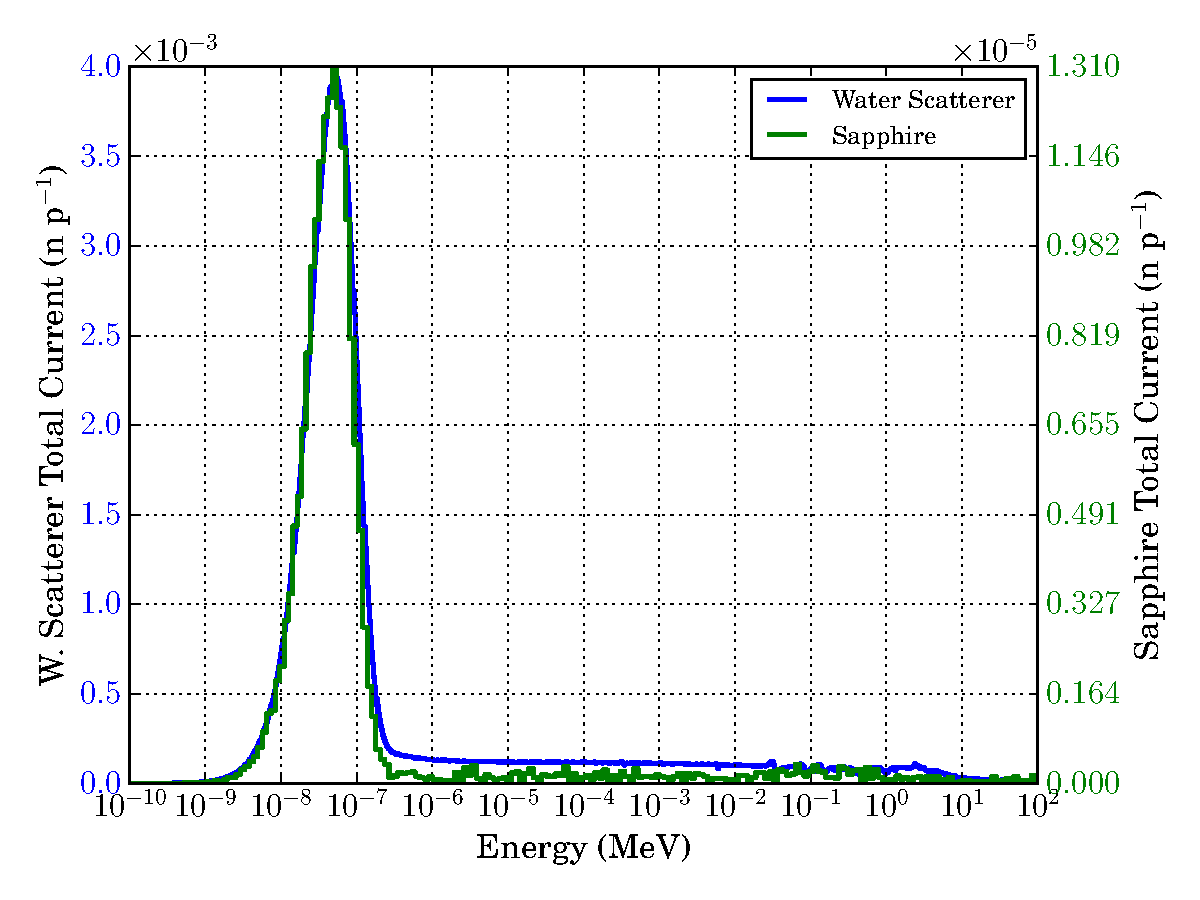
\includegraphics[width=0.33\linewidth]{specs.pdf}%
        %%%%%%%%%%%%%%%%%%%%%%%%%%%%%%%%%%%%%%%%%%%%%%%%%%%%%%%

        %%%%%%%%%%%%%%%%%%%%%%%%%%%%%%%%%%%%%%%%%%%%%%%%%%%%%%%
        \begin{table}
        \end{table}
      \end{block}
      
      \vskip-2ex
      \begin{columns}[t]
        ~~
        \begin{column}{.57\linewidth}
          \begin{block}{Example Results}   
            \noindent{\hskip1cm\textbf{Correct Examples}}        
            \hrule
            \begin{tabular}{@{}>{\small}c@{}>{\small}c@{}>{\small}c@{}>{\small}c}
              IX-1P & \ \ FIND & \ \ SOMETHING-ONE & \ \ BOOK\\
              \textcolor{black}{IX-1P} & \ \ \textcolor{black}{FIND} & \ \ \textcolor{black}{SOMETHING-ONE} & \ \ \textcolor{black}{BOOK}
            \end{tabular}
            \hrule
            \begin{tabular}{@{}>{\small}c@{}>{\small}c@{}>{\small}c@{}>{\small}c@{}>{\small}c@{}>{\small}c@{}>{\small}c@{}>{\small}c}
              JOHN & \ \ FISH & \ \ WONT & \ \ EAT & \ \ BUT & \ \ CAN & \ \ EAT & \ \ CHICKEN\\
              \textcolor{black}{JOHN} & \ \ \textcolor{black}{FISH} & \ \ \textcolor{black}{WONT} & \ \ \textcolor{black}{EAT} & \ \ \textcolor{black}{BUT} & \ \ \textcolor{black}{CAN} & \ \ \textcolor{black}{EAT} & \ \ \textcolor{black}{CHICKEN}
            \end{tabular}
            \hrule
            \begin{tabular}{@{}>{\small}c@{}>{\small}c@{}>{\small}c}
              LOVE & \ \ JOHN & \ \ WHO\\
              \textcolor{black}{LOVE} & \ \ \textcolor{black}{JOHN} & \ \ \textcolor{black}{WHO}
            \end{tabular}
            \hrule
            \begin{tabular}{@{}>{\small}c@{}>{\small}c@{}>{\small}c@{}>{\small}c@{}>{\small}c}
              JOHN & \ \ BUY & \ \ YESTERDAY & \ \ WHAT & \ \ BOOK\\
              \textcolor{black}{JOHN} & \ \ \textcolor{black}{BUY} & \ \ \textcolor{black}{YESTERDAY} & \ \ \textcolor{black}{WHAT} & \ \ \textcolor{black}{BOOK}
            \end{tabular}
            \hrule          
            \vskip2ex
            \noindent{\hskip1cm\textbf{Incorrect Examples}}\par                              
            \hrule
            \begin{tabular}{@{}>{\small}c@{}>{\small}c@{}>{\small}c@{}>{\small}c@{}>{\small}c@{}>{\small}c}
              MARY & \ \ VEGETABLE & \ \ KNOW & \ \ IX & \ \ LIKE & \ \ CORN\\
              \textcolor{black}{MARY} & \ \ \textcolor{black}{VEGETABLE} & \ \ \textcolor{black}{KNOW} & \ \ \textcolor{black}{IX} & \ \ \textcolor{black}{LIKE} & \ \ \textcolor{red}{MARY}
            \end{tabular}
            \hrule
            \begin{tabular}{@{}>{\small}c@{}>{\small}c@{}>{\small}c@{}>{\small}c@{}>{\small}c@{}>{\small}c@{}>{\small}c}
              JOHN & \ \ IX & \ \ GIVE & \ \ MAN & \ \ IX & \ \ NEW & \ \ COAT\\
              \textcolor{black}{JOHN} & \ \ \textcolor{black}{IX} & \ \ \textcolor{red}{WOMAN} & \ \ \textcolor{black}{\underline{\phantom{MAN}}} & \ \ \textcolor{black}{\underline{\phantom{IX}}} & \ \ \textcolor{black}{NEW} & \ \ \textcolor{black}{COAT}
            \end{tabular}
            \hrule
            \begin{tabular}{@{}>{\small}c@{}>{\small}c@{}>{\small}c@{}>{\small}c}
              & \ \ LIKE & \ \ CHOCOLATE & \ \ WHO\\
              \textcolor{green}{JOHN} & \ \ \textcolor{black}{LIKE} & \ \ \textcolor{black}{CHOCOLATE} & \ \ \textcolor{black}{WHO}
            \end{tabular}
            \hrule
            \begin{tabular}{@{}>{\small}c@{}>{\small}c@{}>{\small}c@{}>{\small}c@{}>{\small}c}
              JOHN & \ \ [UNKNOWN] & \ \  & \ \ BUY & \ \ HOUSE\\
              \textcolor{black}{JOHN} & \ \ \textcolor{red}{FUTURE} & \ \ \textcolor{green}{NOT} & \ \ \textcolor{black}{BUY} & \ \ \textcolor{black}{HOUSE}
            \end{tabular}
            \hrule
            \vspace{-1ex}            
          \end{block}
        \end{column}
        ~
        \begin{column}{.4\linewidth}
          \begin{block}{RWTH-BOSTON-104 Database}   
            %%%%%%%%%%%%%%%%%%%%%%%%%%%%%%%%%%%%%%%%%%%%%%%%%%%%%%
            \noindent{\hskip1cm\textbf{Corpus Statistics}}        
            \begin{table}
              \centering
              %\footnotesize
              %\caption{Corpus Statistics}
              \begin{tabular}{@{} p{.5\linewidth}  r r @{}}
                \toprule
                                 & Training   &  Test \\
                \midrule
                sentences        & 161        &  40   \\
                running words    & 710        & 178   \\
                frames           & 12422      & 3324  \\
                vocabulary       & 103        &  65   \\
                singletons       &  27        &   9   \\
                OOV              & -          &   1   \\
                \bottomrule
              \end{tabular}
            \end{table}
            \vskip2ex
            %%%%%%%%%%%%%%%%%%%%%%%%%%%%%%%%%%%%%%%%%%%%%%%%%%%%%%
            \noindent{\hskip1cm\textbf{LM Perplexities}}        
            \begin{table}
              \centering
              %\caption{}
              \begin{tabular}{@{} p{.8\linewidth} r @{}}
                \toprule
                LM type     & $PP$ \\
                \hline
                zerogram    & 106.0 \\
                unigram     & 36.8 \\
                bigram      & 6.7 \\
                trigram     & 4.7 \\
                \bottomrule
              \end{tabular}
            \end{table}
            %%%%%%%%%%%%%%%%%%%%%%%%%%%%%%%%%%%%%%%%%%%%%%%%%%%%%%%
            \vskip2ex
            Database is publicly available
          \end{block}
        \end{column}
      \end{columns}
                
      \begin{block}{Conclusion}
        \begin{itemize}
        \item LVSR system is suitable for vision-based continuous sign language recognition
        \item many of the principles known from ASR can directly be transfered 
        \item important for ASLR: temporal contexts, pronunciation handling, language modelling, and model combination
        \item \alert{outlook:} connection of recognizer output to a
          statistical machine translation system achieved promising
          translation results
        \end{itemize}
        \vspace{-1ex}
      \end{block}
%%%%%%%%%%%%%%%%%%%%%%%%%%%%%%%%%%%%%%%%%%%%%%%%%%%%%%%

    \end{column}
  \end{columns}
\end{frame}

\end{document}


%%%%%%%%%%%%%%%%%%%%%%%%%%%%%%%%%%%%%%%%%%%%%%%%%%%%%%%%%%%%%%%%%%%%%%%%%%%%%%%%%%%%%%%%%%%%%%%%%%%%
%%% Local Variables: 
%%% mode: latex
%%% TeX-PDF-mode: t
%%% End: 